\documentclass[11pt]{article}
\usepackage[margin=1in]{geometry}
\usepackage{amsmath,amssymb,amsthm,booktabs,graphicx,tabularx,microtype}
\usepackage[colorlinks=true,linkcolor=blue,citecolor=blue,urlcolor=blue]{hyperref}
\setlength{\emergencystretch}{2em}
\newtheorem{theorem}{Theorem}
\newtheorem{lemma}[theorem]{Lemma}
\newtheorem{corollary}[theorem]{Corollary}
\newtheorem{conjecture}[theorem]{Conjecture}
\newcommand{\R}{\mathbb R}
\newcommand{\Bcal}{\mathcal B}
\title{Can a Pythagorean Triangle Repeat Its Gravitational Dance?\\
\large Exact Reductions and Partial Results toward the\\
Pythagorean--Burrau Nonperiodicity Conjecture}
\author{Working research draft}
\date{September 5, 2026}
\begin{document}
\maketitle
\begin{abstract}
Release three Newtonian point masses from rest at the vertices of an integer
right triangle, with each mass equal to the length of its opposite side.
Must the resulting motion fail to be collision-free and periodic? We review
the historical experiment, report direct counterexample searches, and develop
partial results toward this conjecture. Exact scaling reduces the integer
family to a rational curve. Time reversal reduces periodicity to a second
simultaneous stop; the Lagrange--Jacobi identity restricts such a stop to a
strict maximum of the moment of inertia. Validated flow covers and a terminal
escape estimate exclude periodicity on a closed interval near $u=0.29$.
Separate endpoint arguments give a punctured near-isosceles interval and
infinitely many thin-triangle escape windows, including a positive-density
subset of an explicit primitive family. Numerical continuation finds nearby
periodic candidates in a larger mass--side family, none satisfying the
right-angle equation. The universal conjecture remains open. We identify a
missing terminal bound in an earlier torque-history argument and retain the
resulting conditional reduction with that hypothesis explicit.
\end{abstract}
\section{A triangle released from rest}\label{sec:intro}

Place three small, perfectly concentrated masses at the corners of a right
triangle. Give the triangle sides of length 3, 4, and 5, and give the bodies
masses 3, 4, and 5, placing each body opposite the side with its own number.
Let go of all three at once. There is no initial push, no friction, and no
force except their mutual Newtonian gravity. What happens?

At first the bodies fall toward one another. Later they can exchange
partners, pass extremely close, or fling one another far away. A particularly
appealing possibility is that they eventually come back to their starting
positions, stop together, and repeat the same dance forever. This paper
asks whether that can happen for \emph{any} integer right triangle when
its masses and opposite sides are tied together in this way. The conjecture
is that it cannot. We have substantial partial results, but no proof of the
universal claim and no counterexample.

\subsection{From Meissel's question to computer experiments}

The starting point is a conversation, rather than a known published
conjecture. In his 1913 paper, Carl Burrau recalled speaking in 1893 with
the Kiel mathematician Ernst Meissel, who believed that the $3$--$4$--$5$
initial conditions would produce periodic motion. Burrau also wanted to
test variable-step numerical integration on a demanding example. His
original account credits Sigurd Kristensen with a substantial part of the
calculation~\cite{Burrau1913}. The attractive integers made the experiment
easy to describe; they did not make its motion easy to calculate.

The decisive revival preceded the famous 1967 publications. Szebehely's
own account records calculations in 1966 by Standish at Yale, Spinelli
with Lecar and Szebehely at NASA's Institute for Space Studies, and Stanek
under Stiefel at ETH Z\"urich. It says that Szebehely suggested the revival,
but does not say how he first encountered Burrau's paper. We have found no
primary-source statement identifying a person or occasion that brought it
to his attention~\cite{Szebehely1967}.

Nor should the intervening years be described as a complete halt in work
on three bodies of comparable masses. Szebehely discusses Str\"omgren's
periodic-orbit work, Zumkley's 1941 integration, and Garcia's 1966 extension
of Zumkley's example~\cite{Szebehely1967}. Zumkley explicitly cites Burrau on the first page of his paper, but
uses three unit masses and a slide rule~\cite{Zumkley1941}. Str\"omgren's
1919 paper likewise studies a different periodic-orbit construction~\cite{Stromgren1919}.
These are related problems, not evidence that the exact $3$--$4$--$5$ trajectory was continuously
recomputed. The sources examined here do not establish a continuation of
that exact calculation between Burrau's work and the documented 1966
revival. This distinction is more defensible than a claim of fifty-four
years of complete silence.

Szebehely and C.~Frederick Peters followed the original motion far enough
to identify its eventual behavior: the two heavier bodies, of masses 4
and 5, form a binary, while the mass-3 body escapes. Their paper explains
that Burrau had stopped at $t=3.35$, before this outcome was apparent.
Their numerical resolution refuted Meissel's expectation for that particular
triangle~\cite{SP1967}. It did not settle every integer right triangle.
In a separate paper that year, they found a nearby periodic solution with
a binary collision and perturbed initial distances~\cite{SPPeriodic}.
That example is outside the collision-free question considered here.

\subsection{The modern question is more specific than free fall}

Starting from rest does not itself rule out periodic motion. Standish's
collisionless periodic example appeared in 1970~\cite{Standish1970}.
Kiyotaka Tanikawa, Hiroaki Umehara, and Hiroshi Abe developed systematic
searches for binary- and triple-collision orbits in 1995; Tanikawa's 2000
continuation studied the structure of this free-fall initial-condition
space~\cite{TUA,Tanikawa2000}. Their work makes collisions part of the
organization of the problem, rather than merely numerical inconveniences.
Moeckel, Montgomery, and Venturelli subsequently developed the rigorous
passage from a configuration at rest to the first collinear configuration,
and constructed periodic collision orbits in the isosceles
problem~\cite{MMV}. Montgomery's \emph{Dropping Bodies} gives a modern
account of periodic free-fall motion and its reversal symmetry~\cite{Montgomery}.
None of these statements identifies the all-integer nonperiodicity claim
of this paper as a conjecture due to Tanikawa or Montgomery.

Recent computations make the distinction still more important. Li and
Liao's 2019 catalogue reports 316 periodic free-fall solutions, including
313 new examples, for several mass ratios~\cite{LiLiao}.
Hristov, Hristova, Dmitra\v sinovi\'c, and Tanikawa's 2024 equal-mass search
reports 12,409 distinct solutions below its specified scale-invariant
period cutoff~\cite{Hristov}. These catalogues vary initial shapes more
freely than our experiment. Equal masses cannot satisfy our right-triangle
mass--side rule. Unequal-mass entries are useful starting guesses, but must
still satisfy both the mass--side relation and the right-angle equation.

The original Pythagorean problem also remains a numerical benchmark:
Rantala, Pihajoki, Mannerkoski, Johansson, and Naab use it to test their
2020 regularized integrator~\cite{Rantala}. Chitan, Myll\"ari, and Haque
revisited Pythagorean black-hole triples in 2022, and Chitan, Myll\"ari,
and Valtonen studied spin effects in 2025~\cite{Chitan2022,Chitan2025}.
Those relativistic extensions address encounters, escape, and mergers under
modified equations. They demonstrate continued interest in the experiment,
while leaving the exact Newtonian conjecture here open.

\subsection{One number specifies the experiment}

The rule ``mass equals opposite side'' is understood in chosen mass and
length units, with gravitational constant set to one. Enlarging all three
masses and all three lengths by the same factor changes the clock rate,
but preserves whether the motion repeats. We can therefore divide by the
hypotenuse and work with a longest side and largest mass equal to one.
Write the two other side lengths, and their corresponding masses, as
$A$ and $B$. The right-angle condition becomes $A^2+B^2=1$.

A convenient way to describe every such triangle is to slide a single
parameter $u$ through the interval $(0,1)$:
\begin{equation}\label{eq:parameter}
 A=\frac{1-u^2}{1+u^2},\qquad B=\frac{2u}{1+u^2}.
\end{equation}
Geometrically, if $(A,B)=(\cos\theta,\sin\theta)$, then
$u=\tan(\theta/2)$. No trigonometry is required to use the rational
formulas. If $u=p/q$ is a fraction in lowest terms, multiplying through
by $q^2+p^2$ gives Euclid's integer triple
\[
 (q^2-p^2,\ 2pq,\ q^2+p^2).
\]
Divide the triple by two when both $p$ and $q$ are odd. Conversely, every
primitive integer right triangle arises this way, allowing exchange of its
two legs. ``Primitive'' means that the three integers have no common
factor. For example, $u=1/2$ gives $(3,4,5)$, and $u=1/3$ gives $(4,3,5)$
after reduction. These are the same experiment with the first two labels
exchanged.

To avoid counting it twice, we use
\[
 0<u\le u_{\rm iso}:=\sqrt2-1,\qquad A\ge B.
\]
Near zero the triangle is very thin; at the other endpoint its two legs are
equal. That equal-leg endpoint has irrational $u$, so it belongs to the
continuous family used in the proof, but not to the integer conjecture.
Changing $u$ changes the masses \emph{and} the shape together. It does not
mean moving one body while keeping three arbitrary masses fixed.

\begin{figure}[tb]
\centering
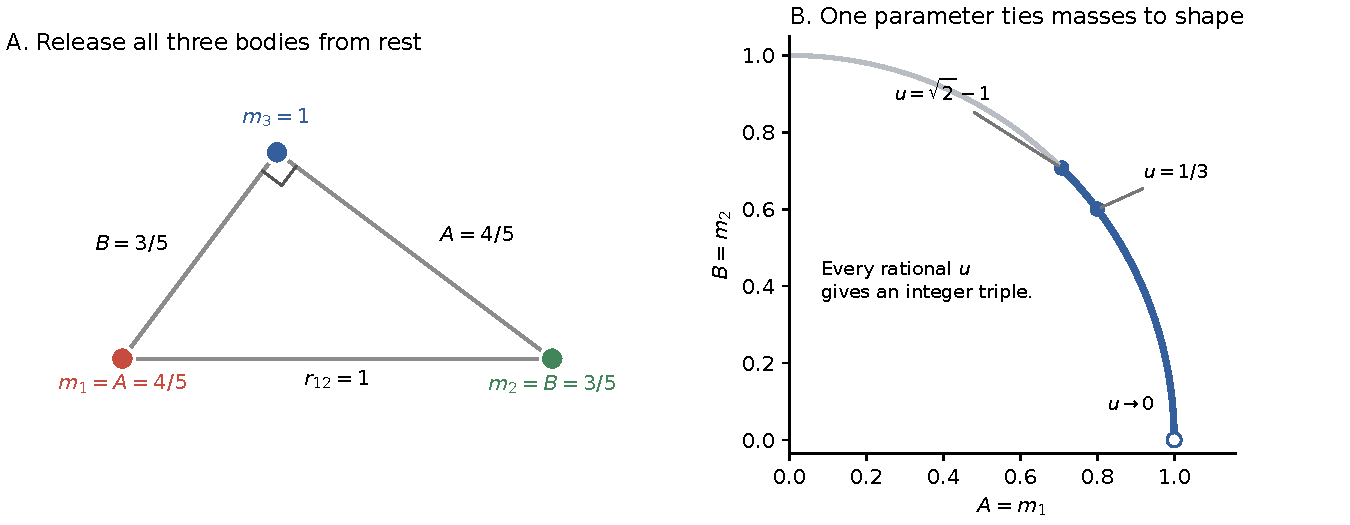
\includegraphics[width=\linewidth]{figures/initial-geometry.pdf}
\caption{The experiment and its parameter. Left: the normalized
$u=1/3$ triangle, with masses $(4/5,3/5,1)$ opposite equal-numbered side
lengths; all velocities initially vanish. Right: the allowed mass pairs
lie on the quarter unit circle. The darker arc is the fundamental interval
$0<u\le\sqrt2-1$; the thin-triangle endpoint $u=0$ is excluded. Rational
$u$, rather than arbitrary points selected numerically on the arc, produces
the integer triples.}
\label{fig:geometry}
\end{figure}

\subsection{What would count as a counterexample?}

A repeating picture is not enough. Each labelled body must return to its
own position with its own velocity in the same fixed coordinate frame,
without any collision along the way. A return after rotating the picture,
swapping bodies, or mathematically continuing through a collision does not
meet this definition. A numerical near-return, however precise, is a
candidate to investigate rather than an exact periodic orbit.

There is a useful simplification. Newton's equations work equally well
backward in time. If a collision-free trajectory that starts at rest ever
stops \emph{all three bodies simultaneously} a second time, it must retrace
its entire path and return to the beginning. Conversely, every periodic
trajectory starting at rest has such a second stop. Mathematicians call a
simultaneous stop a \emph{brake}. The conjecture can therefore be phrased
as: \emph{no integer Pythagorean experiment has a second brake before its
first collision}. Section~\ref{sec:search} describes our direct attempts
to find one.

\subsection{What the proof attempt achieves}

The difficulty is to control every future encounter for infinitely many
triangles. Figure~\ref{fig:fan} shows how nearby rational parameters can
produce visibly similar motion over a finite time, while close approaches
make numerical errors and small changes of parameter matter. A dense plot
is not a proof that a whole interval has been covered.

Three kinds of progress are established by the arguments and certificates
assembled here. First, an exact reduction identifies the only moments at
which a second brake is possible: strict maxima of the system's moment of
inertia, a measure of its overall spread. At such a maximum the changing
triangle still has to stop changing shape. Second, validated integration
and a forward escape estimate exclude every second brake on the explicit
real interval $[0.29,0.2900000101]$. Third, endpoint arguments give a
punctured neighborhood of the equal-leg triangle and infinitely many open
intervals accumulating at the thin-triangle end. On the explicit family
$(4n^2-1,4n,4n^2+1)$, the latter arguments cover a set of indices of positive
lower density: a positive fraction in the limiting lower-density sense,
not necessarily every large index.

These results leave much of the parameter interval unclassified. The
near-equal-leg cutoff is existential, and the thin-triangle result covers
escape windows rather than all phases. We also develop torque-history
identities that could help control the remaining region. The scalar
sign-change shortcut proposed in an earlier draft needs an additional
endpoint bound; Section~\ref{sec:torque} explains the correction. The
paper's outcome is a set of rigorous reductions and partial exclusions,
with the remaining global obligation stated explicitly.

\begin{figure}[p]
\centering
\begin{minipage}[c][.75\textheight][s]{.24\linewidth}
\raggedleft\small
\vspace*{.045\textheight}
$\Delta u=10^{-2}$\par\vfill
$\Delta u=10^{-2.5}$\par\vfill
$\Delta u=10^{-3}$\par\vfill
$\Delta u=10^{-3.5}$\par\vfill
$\Delta u=10^{-4}$\par
\vspace*{.065\textheight}
\end{minipage}\hspace{1em}%
\raisebox{-.5\height}{
\includegraphics[height=.75\textheight]{figures/oklo_pythagorean_fan_trajectory_progression.png}}
\caption{Progressively narrower collections of integer experiments near
$u=0.29$, using the project's original fan--trajectory visualization.
From top to bottom the intervals are $[0.29,0.29+\Delta u]$, with
$\Delta u=10^{-2},10^{-2.5},10^{-3},10^{-3.5},10^{-4}$.
Each left panel displays 400 primitive triples of smallest hypotenuse in
its interval, with radius on a common affine $\log_{10}c$ scale and its
angular interval expanded to one display radian. The highlighted sector
is the next narrower interval; large rings select ten triples whose
trajectories appear at right. Red, green, and blue track the three bodies
in the source plot's leg ordering. Right panels share one spatial scale,
show normalized physical times $0\le t\le4$, and clip outgoing paths.
Opacity decreases with body speed; it is not an integration-error measure.
Even the narrowest displayed interval is about 9,901 times wider than the
certified interval. This ordinary numerical illustration conveys the
search geometry, not validated parameter coverage.}
\label{fig:fan}
\end{figure}

\section{Attempts to construct a counterexample}\label{sec:search}

The search starts from an adversarial question: can a known periodic
free-fall orbit be adjusted until it lies exactly on the Pythagorean
curve? This is more directed than waiting for a long trajectory to nearly
return. It also tests whether the apparent scarcity of second brakes is
merely an artifact of sampling.

\subsection{Impose the geometric constraints in stages}

Normalize $m_3=r_{12}=1$. In the larger family where each mass equals its
opposite side, a valid nondegenerate triangle has
\begin{equation}\label{eq:general-tied}
 q_1=(-1/2,0),\quad q_2=(1/2,0),\quad
 q_3=(x,y),\quad
 x={m_2^2-m_1^2\over2},\quad
 y=\sqrt{m_2^2-(x+1/2)^2}>0.
\end{equation}
There are now two adjustable mass ratios. Periodic candidates in this
larger family need not be right triangles. Their remaining defect is
\begin{equation}\label{eq:defect}
 D=m_1^2+m_2^2-1.
\end{equation}
An exact zero of $D$ is required even to challenge the stronger conjecture
for real parameters. An integer counterexample additionally needs rational
$u=m_2/(1+m_1)$.

Our September 2026 campaign starts from six entries of Li and Liao's
unequal-mass catalogue~\cite{LiLiao}. In the numerical construction we solve
three independent second-brake equations together with two mass--side
matching equations, varying the two initial-position coordinates, two
mass ratios, and a regularized flight time. Levi--Civita coordinates
replace the selected pair separation by a complex square and slow the
clock near close approaches. An atlas of pair choices avoids relying on
one coordinate chart for every encounter. Analytic variational equations
supply the shooting derivatives; pseudo-arclength continuation recovers
seeds for which direct correction stalls.

\begin{table}[tb]
\centering
\small
\begin{tabular}{lrrrr}
\toprule
Seed & $m_1$ & $m_2$ & Second-brake time & $D$\\
\midrule
$F_1$ & .536940689 & .839991651 & 1.337970014 & $-.006108723$\\
$F_2$ & .485763526 & .878297063 & 1.413330015 & $+.007371934$\\
$F_3$ & .343754597 & .887462426 & 1.074865097 & $-.094243220$\\
$F_4$ & .335421060 & .903827720 & 1.133475174 & $-.070588165$\\
$F_5$ & .474742622 & .896107795 & 1.544076262 & $+.028389737$\\
$F_{30}$ & .594811647 & .801774973 & 6.289233824 & $-.003355997$\\
\bottomrule
\end{tabular}
\caption{Ordinary numerical periodic candidates in the larger
mass--opposite-side family. None is Pythagorean. Digits are displayed for
reproducibility, not as interval-certified enclosures. The flight time is
physical normalized time; twice this value would be a period at an exact
collision-free second brake. Seed names refer to catalogue origins, not
to established connected branches of solutions.}
\label{tab:candidates}
\end{table}

\begin{figure}[tb]
\centering
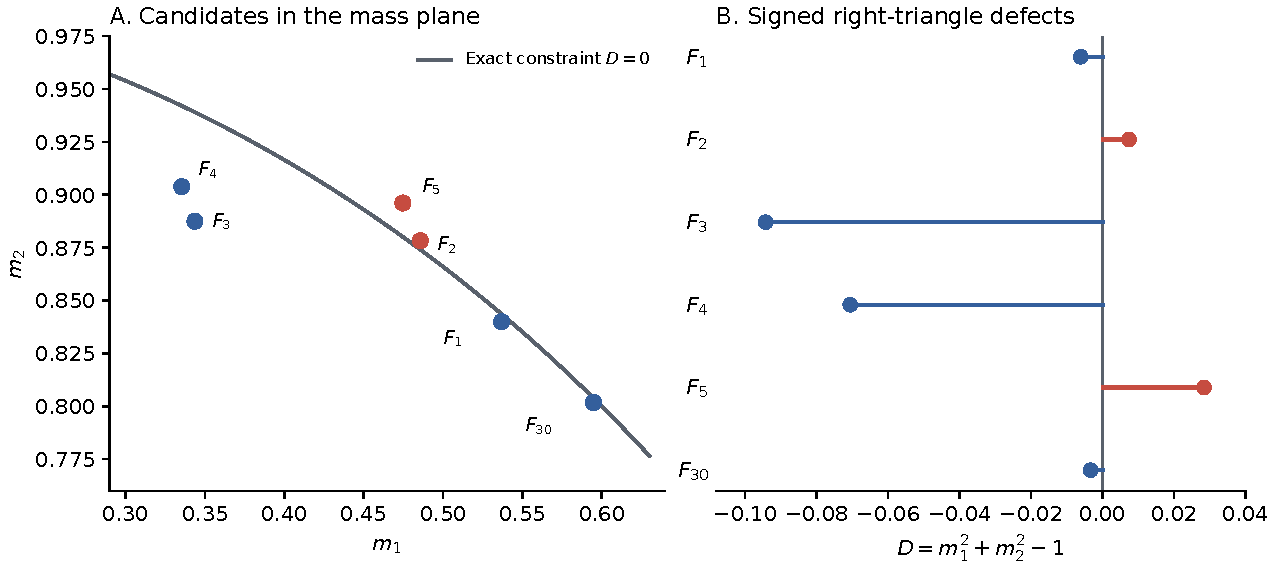
\includegraphics[width=.9\linewidth]{figures/counterexample-defects.pdf}
\caption{The six numerical candidates of Table~\ref{tab:candidates} and
exact right-triangle constraint. The left panel places them relative to
$m_1^2+m_2^2=1$; the right displays each signed defect directly. Opposite
signs at unrelated candidates are not an intermediate-value bracket.
No connecting solution branch is established by these points.}
\label{fig:defects}
\end{figure}

\subsection{What the numerical checks establish}

The corrected shooting residuals are at most about $1.2\times10^{-12}$.
Reintegration with an implicit Radau method, comparison with DOP853, and
backward reversal reproduce the candidate states to roughly
$2\times10^{-12}$. The corresponding five-equation Jacobians have
ordinary smallest singular values between approximately $0.199$ and
$0.870$ in the recorded physical-parameter convention. Their numerical
nonsingularity suggests isolated solutions of the five matching equations,
rather than freely adjustable families that automatically cross $D=0$.
It does not prove existence or isolation: those conclusions require a
validated implicit-function calculation.

The closest sampled separations range from about $3.4\times10^{-6}$ to
$5.0\times10^{-4}$. These values explain the use of regularization and
also limit the evidence: sampling alone does not certify positive
separation for every intervening time. Reconstructed energy is especially
sensitive to cancellation near the deepest passages; the campaign's worst
sampled physical energy error is about $2.5\times10^{-7}$. Small shooting
residuals must not be presented as equally small error bounds for every
physical observable.

We separately impose the exact right-triangle parameterization and look
for small kinetic energy at local maxima of the moment of inertia. Four
local searches seeded from $F_1,F_2,F_3,F_5$ converge to positive minima,
the smallest about $1.28\times10^{-4}$. The $F_{30}$ search reaches its
evaluation limit and remains noise-limited; the $F_4$ event correction
leaves the required strict-maximum branch. Neither incomplete search is
an exclusion theorem. No exact right-triangle second brake was found, so
there is no candidate on which rational reconstruction would be warranted.
Machine-readable results and exact replay commands accompany the campaign
report listed in Appendix~\ref{sec:reproduction}.

\subsection{Two tempting continuation arguments that do not suffice}

The defects of $F_1$ and $F_2$ have opposite signs. This would be useful if
we had a connected collision-free periodic branch joining them, on which
$D$ varied continuously. We do not. Their labelled half-orbit syzygy
sequences are different, and at zero angular momentum a noncollinear
collision-free orbit crosses every syzygy transversely. Consequently those
finite sequences cannot change on a connected finite-flight-time brake
family without an excluded event or endpoint. Opposite defects alone are
not a bracket.

Nor does a rank deficiency automatically construct the missing branch.
For five smooth equations in five unknowns, a rank-four Jacobian leaves
one direction to inspect, but the remaining scalar equation after
Lyapunov--Schmidt reduction can be $s^2=0$, with an isolated root. A branch
requires that residual equation to vanish along the proposed continuation.
Similarly, raw free-group words from the catalogue do not distinguish
these brake loops: a full brake orbit retraces its path and its loop in
collision-free shape space is null-homotopic. The ordered, labelled
syzygy sequence is the useful finite-itinerary information here.

The search has therefore produced well-tested near misses and sharper
requirements for a counterexample. It has not supplied a probability of
nonexistence, a numerical proof of the conjecture, or an obstruction to
unsearched long-period families.

\section{The exact problem and its reductions}\label{sec:exact}

Let $a^2+b^2=c^2$ with positive integers, set
$(m_1,m_2,m_3)=(a,b,c)$, and put
\[
q_1=(-c/2,0),\quad q_2=(c/2,0),\quad
q_3=((b^2-a^2)/(2c),ab/c),\qquad \dot q_i=0.
\]
The side opposite each mass has the same length as that mass.  We work with $G=1$ and the equations
\[
 \ddot q_i=\sum_{j\ne i}m_j{q_j-q_i\over|q_j-q_i|^3}.
\]
\begin{conjecture}[Pythagorean--Burrau nonperiodicity]
For every positive integer triple $a^2+b^2=c^2$, the solution with these
initial data has no collision-free labelled period.
\end{conjecture}
A labelled period is an exact return in the fixed inertial frame. The
maximal classical solution ends at its first collision; regularized
continuation through that collision is a different notion of solution.

\subsection{Scaling and the rational parameter curve}

\begin{lemma}[Simultaneous mass--length scaling]
If $q_i(t)$ solves the equations with masses $m_i$, then for $k>0$
\[
\widetilde m_i=km_i,\qquad \widetilde q_i(t)=kq_i(t/k)
\]
solves the rescaled problem.  A labelled period $T$ corresponds exactly to a
period $kT$.
\end{lemma}
\begin{proof}
Both sides of Newton's acceleration equation acquire the factor $k^{-1}$.
Velocity is unchanged after the corresponding time substitution, and mutual
distances acquire the positive factor $k$.
\end{proof}

It follows that only primitive triples matter.  For $u\in(0,1)$ define
\[
A(u)=\frac{1-u^2}{1+u^2},\qquad
B(u)=\frac{2u}{1+u^2}.
\]
If $u=p/q$ is reduced, Euclid's integer triple is
$(q^2-p^2,2pq,q^2+p^2)$ and its common divisor is two exactly when $p,q$ are
both odd.  Conversely Euclid's theorem recovers every ordered primitive
triple.  The inverse is $u=B/(1+A)$, and leg exchange is the involution
$u\mapsto(1-u)/(1+u)$.  Its fixed point is $\sqrt2-1$, giving the fundamental
interval $0<u\leq\sqrt2-1$ for the real family.

After normalizing $c=1$, masses and positions are
\[
(A,B,1),\qquad q_1=(-1/2,0),\quad q_2=(1/2,0),\quad
q_3=((B^2-A^2)/2,AB).
\]
We call this one-parameter family \emph{tied}, since its masses and initial
opposite sides vary together. The stronger real conjecture makes the same
nonperiodicity assertion for every $0<u\le\sqrt2-1$.

\subsection{Initial geometry}

The initial center of mass is the incenter: both have barycentric weights
equal to the opposite side lengths. The identity
$I=(\sum m_i)^{-1}\sum_{i<j}m_im_jr_{ij}^2$ gives, directly,
\[
 I_0=abc,\qquad U_0={ab\over c}+{ac\over b}+{bc\over a}.
\]
In the normalized problem,
\[
 I_0=AB,\qquad U_0=AB+(AB)^{-1},\qquad H=-U_0.
\]
Here $I$ is the moment of inertia about the center of mass and $U$ is the
positive potential magnitude. The right angle is not preserved: for
$D=r_{12}^2-r_{23}^2-r_{31}^2$,
\[
 D(0)=\dot D(0)=0,\qquad
 \ddot D(0)=2\bigl[(AB)^{-1}-AB(A+B)\bigr]>0.
\]
Thus the angle opposite $r_{12}$ initially becomes obtuse. This local sign
does not define an invariant region; numerical integration at $u=1/3$
finds later changes of sign of $D$.

\subsection{Second brakes and a residual valid at collinearity}

\begin{lemma}[Second-brake lemma]
A classical free-fall segment generates a collision-free labelled periodic
solution if and only if all inertial velocities vanish at some positive time
before collision.
\end{lemma}
\begin{proof}
Uniqueness and time reversal give $q(-t)=q(t)$.  A brake at $\tau$ gives
$q(\tau+s)=q(\tau-s)$ and hence a labelled period $2\tau$.  Conversely, a
labelled period $T$ combined with the symmetry at zero gives reflection
symmetry about $T/2$, and therefore zero velocity there.  The period $2\tau$
need not be minimal unless $\tau$ is the first positive brake.
\end{proof}

Write $r_{ij}=|q_j-q_i|$, $K=\tfrac12\sum_i m_i|\dot q_i|^2$,
$U=\sum_{i<j}m_im_j/r_{ij}$, and $H=K-U=-U_0$. In the center-of-mass
frame define reduced masses $\mu_1=m_1m_2/(m_1+m_2)$ and
$\mu_2=m_3(m_1+m_2)/(m_1+m_2+m_3)$, and Jacobi vectors
\[
X=q_2-q_1,\qquad
Y=q_3-\frac{m_1q_1+m_2q_2}{m_1+m_2}
\]
and Hopf invariants
\[
h(X,Y)=\left(\frac{|X|^2-|Y|^2}{2},X\cdot Y,X\times Y\right).
\]
We use the quotient residual
\[
\Bcal(u,t)=\frac{d}{dt}h(X(u,t),Y(u,t)).
\]
Away from triple collision, $Dh$ has rank three and kernel equal to the common
rotation direction.  Since total linear and angular momentum vanish,
$\Bcal=0$ is equivalent to vanishing of every labelled inertial velocity.
Unlike three mutual-distance derivatives, this remains true at syzygy.
Indeed, a velocity in $\ker Dh$ has the form
$(\dot X,\dot Y)=\omega(iX,iY)$, whose angular momentum is $\omega I$;
$L=0$ and $I>0$ force $\omega=0$.

For an explicit configuration-space reduction, rotate with $X$ and write
$X=(R,0)$, $Y=(C,D)$. Eliminating the common rotation at $L=0$ gives
\[
 K_{\rm red}={\mu_1\dot R^2+\mu_2(\dot C^2+\dot D^2)\over2}
 -{\mu_2^2(C\dot D-D\dot C)^2\over
 2[\mu_1R^2+\mu_2(C^2+D^2)]}.
\]
Here the dots on $C,D$ differentiate coordinates in the moving frame.
Substitution of
$\dot\theta=-\mu_2(C\dot D-D\dot C)/I$ into the inertial kinetic
energy proves the formula. With $m_{12}=m_1+m_2$, the potential is
\[
 U={m_1m_2\over R}
 +{m_1m_3\over\sqrt{(C+m_2R/m_{12})^2+D^2}}
 +{m_2m_3\over\sqrt{(C-m_1R/m_{12})^2+D^2}}.
\]
The tied brake curve is
$R=1$, $C=AB(B-A)/(A+B)$, $D=AB$, with zero reduced velocity.

\section{Finite certificates for nonperiodicity}\label{sec:events}

Let
\[
 I=\mu_1|X|^2+\mu_2|Y|^2,\qquad
 \sigma=\mu_1\overline X\dot X+\mu_2\overline Y\dot Y,
 \qquad
 \zeta=\mu_1\overline X\dot X-\mu_2\overline Y\dot Y .
\]
Here complex multiplication identifies the oriented plane with $\mathbb C$.
Then $\dot I=2\operatorname{Re}\sigma$ and the angular momentum is
$L=\operatorname{Im}\sigma$.  Consequently, at $L=0$ and away from $Y=0$,
\[
 \dot I=0\ \hbox{ and }\ \zeta=0
 \quad\Longleftrightarrow\quad
 \dot X=\dot Y=0.
\]
The implication from a brake to these three scalar equalities is
unconditional.  At the Jacobi degeneracy $Y=0$, the Hopf residual $\Bcal$
above supplies the coordinate-independent converse.

This splitting has an exact shape interpretation.  Put
$J_X=\mu_1|X|^2$, $J_Y=\mu_2|Y|^2$, $s=J_X/I$, and
$\phi=\arg Y-\arg X$.  At every zero of $\dot I$ with $X,Y\ne0$ and $L=0$,
\[
 \boxed{\quad
 \zeta=I\left(\dot s-2is(1-s)\dot\phi\right),\qquad
 |\zeta|^2={8KJ_XJ_Y\over I}=8KI\,s(1-s).
 \quad}
\]
Indeed $\sigma=0$ gives
$\zeta=2\mu_1\overline X\dot X=-2\mu_2\overline Y\dot Y$; decomposing each
Jacobi velocity into radial and angular parts proves both formulas.  Thus a
maximum event is a brake exactly when its shape velocity vanishes, and the
origin-avoidance problem can equivalently be written as the scalar strict
inequality $K=U-U_0>0$. At a brake time $\tau$, time reversal gives
\[
 K(\tau+s)={s^2\over2}\sum_i m_i|\ddot q_i(\tau)|^2+O(s^4).
\]
The coefficient is positive, since $\ddot I(\tau)=-2U_0<0$ rules out
vanishing of all accelerations. A brake is consequently a quadratic zero
of $K$ in time, which cannot be detected by a sign change of $K$.

There is also a brake residual intrinsic to any binary Levi--Civita chart.
For a selected pair write $g=q_j-q_i=w^2$, $dt=|w|^2d\sigma$, and
$z=dw/d\sigma$. Let $G$ be the third body relative to the selected pair's
center of mass and $P=\dot G$. With reduced masses $\mu_g,\mu_G$, angular
momentum is
\[
 L=2\mu_g\operatorname{Im}(\overline w z)+\mu_G G\times P.
\]
Thus, on a collision-free zero-angular-momentum trajectory and wherever
$G\ne0$,
\[
 \boxed{\quad (z_r,z_i,G\cdot P)=0
 \quad\Longleftrightarrow\quad\hbox{a labelled brake}.\quad}
\]
Indeed $z=0$ gives $\dot g=0$; then $L=0$ gives $G\times P=0$, while
$G\cdot P=0$ forces $P=0$. Total momentum removes the common translation.
This residual stays regular through arbitrarily close selected-pair
passages; at $G=0$ one changes Jacobi tree or uses $\Bcal$.

\begin{theorem}[Brake-event identities]
Along a collision-free free-fall solution with initial potential $U_0$, every
brake satisfies
\[
 K=0,\qquad U=U_0,\qquad \ddot I=-2U_0<0,
 \qquad r_{ij}\geq {m_im_j\over U_0}.
\]
At any zero of $\dot I$ for which $\ddot I\geq0$, one instead has
$K\geq U_0$.
\end{theorem}
\begin{proof}
With positive potential magnitude $U$ and energy $H=K-U=-U_0$, the
Lagrange--Jacobi identity is
\[
 \ddot I=4K-2U=2K-2U_0=2U-4U_0.
\]
At a brake $K=0$, giving the first three assertions.  Since every summand
$m_im_j/r_{ij}$ is positive and bounded above by $U=U_0$, the separation
bound follows.  If $\ddot I\geq0$, the middle expression instead gives
$K\geq U_0$.
\end{proof}

\begin{corollary}[Validated-cover criterion]\label{cor:cover}
Suppose a classical free-fall solution has a launch window $[0,t_L]$ on
which $U<2U_0$. Suppose validated flow enclosures cover every time in
$[t_L,t_*]$, and every enclosure proves at least one of
\[
 \dot I\ne0,\qquad K>0,\qquad \Bcal\ne0.
\]
Then there is no second brake in $(0,t_*]$. If the terminal enclosure
satisfies a proved forward collision-or-escape criterion that excludes every
later brake, the initial free-fall solution is nonperiodic.
\end{corollary}
\begin{proof}
At launch $\dot I(0)=0$, whereas $U<2U_0$ implies $\ddot I<0$.
Consequently $\dot I(t)<0$ for $0<t\le t_L$. The remaining disjunction
excludes a brake at every covered time. This argument applies fiber by fiber
when $t_*$ depends on a parameter; both section images and the complete
intervening flow tubes must be covered. The initial brake itself is never
subjected to the nonvanishing disjunction.
\end{proof}

This criterion has been implemented with exact rational initial data and
MPFR interval arithmetic.  The archived certificates prove the conjecture
for
\[
(21,20,29),\ (5311,5280,7489),\ (8319,8200,11681),
\ (33439,32400,46561),\ (72,65,97)
\]
in both leg orderings. The parameter-cover results below require additional
control of how the enclosed trajectories depend on $u$.

\begin{lemma}[Terminal escape certificate]\label{lem:escape}
For a prospective binary of total mass $M$ and an outer body of mass $m_c$,
let $x,y$ be the inner and outer Jacobi vectors, $r=|x|$, $\rho=|y|$, and
$e=|\dot x|^2/2-M/r$. Choose $\eta>0$, set $R=M/\eta$ and
$s_0=\rho_0-R$, and suppose
\[
s_0>0,\quad \dot\rho_0>0,\quad
\delta=\frac12\dot\rho_0^2-\frac{M+m_c}{s_0}>0,
\]
\[
e_0+\frac{m_c\sqrt{2MR}}
{\sqrt{2\delta}\,s_0^2}<-\eta.
\]
Then the future solution either ends in inner binary collision or the outer
body escapes with $\dot\rho\ge\sqrt{2\delta}$ forever. In particular there is
no later classical brake.
\end{lemma}
\begin{proof}
On the bootstrap region $e<-\eta$, one has
$r<R$ and $r|\dot x|<\sqrt{2MR}$. The Newton field derivative bound
$\|D(v/|v|^3)\|\le2/|v|^3$ gives
\[
|\dot e|\le\frac{2m_cr|\dot x|}{(\rho-r)^3}.
\]
The outer Jacobi acceleration obeys
$|\ddot y|\le(M+m_c)/(\rho-r)^2$, so
$\ddot\rho\ge-(M+m_c)/(\rho-R)^2$. Therefore
\[
J=\frac12\dot\rho^2-\frac{M+m_c}{\rho-R}
\]
is nondecreasing while $\dot\rho>0$. Its initial value $\delta>0$
prevents $\dot\rho$ from reaching zero. Hence
$\rho\ge\rho_0+\sqrt{2\delta}(t-t_0)$, and the total future tidal increase of
$e$ is at most the allowance in the hypothesis. Its strict margin closes the
bootstrap. The positive gap $\rho-r$ excludes an outer collision; only an
inner binary collision can terminate the resulting escape trajectory.
\end{proof}

The near-triple-collision scaling below has limiting inner energy zero,
so it requires an escape criterion that permits an expanding inner pair.

\begin{lemma}[Escape with a possibly expanding inner pair]\label{lem:hierarchical}
Use the same Jacobi variables, let $w_0=\rho_0-r_0>0$, and choose
$\varepsilon,c>0$. Put
\[
 v_b=\sqrt{2M/r_0+2\varepsilon},\qquad
 \mathcal T=\int_0^\infty
 {\sqrt{2M(r_0+v_bt)+2\varepsilon(r_0+v_bt)^2}
  \over(w_0+ct)^3}\,dt.
\]
If
\[
 \dot\rho_0-{M+m_c\over cw_0}>v_b+c,\qquad
 e_0+2m_c\mathcal T<\varepsilon,
\]
then, until a possible inner collision,
$r(t)\le r_0+v_bt$, $\dot\rho(t)>v_b+c$, and
$\rho(t)-r(t)\ge w_0+ct$. In particular there is no later brake.
\end{lemma}
\begin{proof}
Assume $e<\varepsilon$ and $\rho-r\ge w_0+ct$ on a bootstrap interval.
At a first outward crossing of $r_0+v_bt$, the energy inequality gives
$\dot r\le|\dot x|<v_b$, excluding that crossing. Integration of
$\ddot\rho\ge-(M+m_c)/(w_0+ct)^2$ then gives
$\dot\rho>v_b+c$ and preserves the gap. Finally
$r|\dot x|\le\sqrt{2Mr+2\varepsilon r^2}$ bounds the total tidal
increase of $e$ by $2m_c\mathcal T$. The integral converges, and the
strict energy margin closes the bootstrap.
\end{proof}

\begin{theorem}[Validated middle first-maximum interval]
For every real
\[
 {29\over100}\le u\le {14501\over50000},
\]
the tied classical trajectory is collision-free through its first positive
local maximum of $I$, and this maximum is not a labelled brake.  The unique
intervening minimum and the first subsequent maximum obey
\[
 t_{\min}\in[0.758038,0.758045],\qquad
 t_{\max}\in[1.32908,1.33943].
\]
\end{theorem}
\begin{proof}
The exact tied launch is embedded as a one-dimensional mean-value graph with
$u$ retained as a frozen state coordinate.  A pinned MPFR/CAPD $C^1$
Poincare calculation propagates this graph first in a pair--13
Levi--Civita chart and, after an exact Jacobi-tree transformation at $t=1$,
in a pair--23 chart.  On every accepted-step enclosure, all three mutual
separations are strictly positive.  The launch-concavity window and whole-leg audits give $\dot I<0$ after
launch to the first minus-to-plus zero and $\dot I>0$ from that zero to the
first later plus-to-minus zero.  At the minimum,
$U/U_0\in[5.17942,5.18335]$; at the maximum,
$U/U_0\in[0.983016,1.01907]\subset(0,2)$, proving both events strict by
Lagrange--Jacobi.  In the final selected-pair chart the validated residual
has
\[
 \operatorname{Im}z\in[-0.0500738,-0.0113187],\qquad
 P_x\in[-0.0561842,-0.00917817].
\]
A labelled brake forces $z=P=0$, so either strict component excludes it.
Two abutting tiles cover the stated interval. The exact chart identities,
logs, and an independent left-tile replay are indexed in
Appendix~\ref{sec:reproduction}.
\end{proof}

This theorem excludes only the first positive maximum.  It does not rule out
a brake on a later maximum branch and therefore is not, by itself, a
nonperiodicity theorem on the displayed interval.

\begin{theorem}[Validated middle real interval]
For every real
\[
 {29\over100}\le u\le {2900000101\over10000000000},
\]
the tied maximal classical solution has no second labelled brake at any
collision-free time and hence is not a classical periodic solution.
Consequently the Pythagorean--Burrau conjecture holds for infinitely many
primitive triples in this interval, including
$(9159,5800,10841)$ at $u=29/100$.
\end{theorem}

More explicitly, for every integer $k\ge99010$ set
\[
 u_k={290k+1\over1000k}={29\over100}+{1\over1000k}.
\]
The numerator and denominator are coprime and of opposite parity, and the
interval inequality is equivalent to $1/(1000k)\le101/10^{10}$.  The theorem
therefore proves nonperiodicity for the primitive triples
\[
 \left(915900k^2-580k-1,
       580000k^2+2000k,
       1084100k^2+580k+1\right),
 \qquad k\ge99010.
\]
\begin{proof}
A pinned MPFR/CAPD propagation embeds the exact launch curve on
$[0.29,0.290000001]$ in one correlated tripleton with $u$ frozen as a state
coordinate.  Before the
exchange, every accepted full-step enclosure is checked for three positive
mutual separations. The launch window verifies $U<2U_0$; subsequent windows
verify the brake-exclusion disjunction of Corollary~\ref{cor:cover}.  Three algebraic changes of Levi--Civita chart use rigorous
mean-value images.

Across the exchange, six $C^1$ Poincare maps project onto the transverse
pair--13 sections
\[
 w_r=-{3\over5},-{1\over2},-{2\over5},-{3\over10},-{1\over5},0.
\]
For each map a convex mean-value domain contains the propagated family and
its stored center, the validated section derivative transports the
distinguished parameter generator, and an independent $C^0$ integration
covers the complete incoming tube through the latest possible return.
Thus section reconditioning does not omit any inter-section time.  Every
tube enclosure retains positive separation and excludes a brake.

For the terminal binary $\{2,3\}$ set $M=B+1$, $G=q_1-C_{23}$,
$\rho=|G|$, $h=|\dot q_3-\dot q_2|^2/2-M/r_{23}$, and
\[
 R=M/4,\quad d=\rho-R,\quad
 E_\rho={\dot\rho^2\over2}-{A+B+1\over d},\quad
 \Delta={A\sqrt{2MR}\over\sqrt{2E_\rho}\,d^2}.
\]
These are precisely the quantities of Lemma~\ref{lem:escape}; $h$ is
transported as a regularized state variable. Hence the terminal check can
use its enclosure without dividing by the small inner separation.
The resulting terminal enclosure has
\[
\begin{split}
t_*&\in[4.30030837364,4.30032429905],\\
d&>1.8655,\qquad \dot\rho>2.0484,\qquad E_\rho>0.8223,\\
h&<-9.2745,\qquad -4-h-\Delta>5.0690 .
\end{split}
\]
These are the strict hypotheses of Lemma~\ref{lem:escape}
with binary $\{2,3\}$, escaper body 1, and $\eta=4$.  Hence after $t_*$ the
inner pair either collides classically, ending the maximal classical
solution, or body 1 escapes permanently; neither alternative permits a later
brake. The second-brake lemma proves nonperiodicity. A separate interval
checker verifies the terminal inequalities on an outward-widened box;
an independent MPFR replay reproduces the section audits and escape margin.

The remaining extension is the union of 100 independently certified,
adjacent closed tiles of exact width $10^{-10}$, beginning at
$0.2900000001$ and ending at $0.2900000101$.  Every requested interval is
identical to its PASS interval, every consecutive pair shares its exact
rational endpoint, and all 100 full logs are archived. The campaign overlaps
the initial tile, and their union is exactly the stated closed interval.
\end{proof}

This continuum theorem covers a width of $1.01\times10^{-8}$. Larger
parameter covers remain a separate validation problem; experimental wider
propagations are not included in its conclusion.

At a possible brake, the bound $r_{ij}\ge m_im_j/U_0$ is uniform on every
compact parameter interval bounded away from $u=0$. It gives no lower
bound on separations between brake events and degenerates as $u\to0$.

On any regular strict-maximum branch, the implicit-function theorem locally
gives $t=t_k(u)$.  The unresolved condition becomes the planar
origin-avoidance problem
\[
 u\longmapsto \zeta(u,t_k(u))\in\mathbb C\setminus\{0\}.
\]
To turn this into a universal theorem one must also control branch creation,
collision and escape endpoints, degenerate events, and the possible number
of branches.  The nominal dimension count alone supplies none of these
facts.

Numerical diagnostics at $u=1/3$ place maximum-event values of $\zeta$ in
all four quadrants, with the origin in the convex hull of three early
values. These data argue against a fixed real linear projection with one
strict sign at every maximum. Branch-dependent order or a nonlinear
constraint remains a possible approach.

\section{The equal-leg endpoint and its neighbors}\label{sec:iso}

\begin{theorem}
At $u=\sqrt2-1$, the classical solution has no positive second brake and
reaches a binary or triple collision in finite time.
\end{theorem}
\begin{proof}
Here $m_1=m_2=m=1/\sqrt2$ and reflection symmetry persists.  Write the base
bodies as $(-x,y_b),(x,y_b)$ and the apex as $(0,y_a)$, with
$h=y_a-y_b$.  Then
\[
\ddot x=-\frac{m}{4x^2}-\frac{x}{(x^2+h^2)^{3/2}}<0.
\]
Starting with $x_0=1/2$ and $\dot x(0)=0$ gives $\dot x<0$, excluding a
second brake.  While $x>0$, one has
$\ddot x\leq-m/(4x_0^2)$, whence
\[
x(t)\leq x_0-\frac{m}{8x_0^2}t^2.
\]
Thus collision occurs no later than $\sqrt{8x_0^3/m}=2^{1/4}$.
\end{proof}

To study nearby rational parameters, we use the Levi--Civita continuation
of the symmetric orbit as a comparison solution. A collision of a nearby
physical trajectory still terminates its classical motion.

Put $v=u/(\sqrt2-1)$, $(m,n)=(A,B)$, $g=q_2-q_1=w^2$, and
$G=q_3-C_{12}$. With $dt=|w|^2d\sigma$, write $z=w_\sigma$, $P=\dot G$,
and $e=|\dot g|^2/2-(m+n)/|g|$. The selected pair collision is $w=0$;
this is regular in the comparison equations, but it still terminates the
classical trajectory at $v=1$.

For $d_{31}=G+ng/(m+n)$, $d_{23}=G-mg/(m+n)$, and
$F=d_{23}/|d_{23}|^3-d_{31}/|d_{31}|^3$, the regular equations are
\[
\begin{aligned}
 w_\sigma&=z,&
 z_\sigma&={e\over2}w+{|w|^2\bar w\over2}F,&
 e_\sigma&=2\operatorname{Re}(wz\bar F),\\
 G_\sigma&=|w|^2P,&
 P_\sigma&=-|w|^2{m+n+1\over m+n}
 \left({m d_{31}\over|d_{31}|^3}+{n d_{23}\over|d_{23}|^3}\right).
\end{aligned}
\]
They preserve $2|z|^2-(m+n)-e|w|^2=0$ and are analytic at $w=0$
when the other two separations are positive. At $v=1$ the launch is
$(w,z,e,G,P)=(1,0,-\sqrt2,i/2,0)$; its only nonzero parameter
derivatives are
$m_v=-1/2$, $n_v=1/2$, and $G_{x,v}=1/(2\sqrt2)$.

\subsection{The initial arc and collision unfolding}

The first syzygy, or collinear configuration, is reached without a brake
for all tied parameters sufficiently near $v=1$. The relevant variational
argument also establishes the torque inequality used in
Section~\ref{sec:torque}. Write
$F_0(v,t)=\eta(v,t)-h(v,t)$ for the history-threshold difference defined
there, and let $\tau(v)$ be the first syzygy time. On the symmetric orbit,
$F_0(1,t)=0$. Differentiation of the Newtonian equations and the exact
tied launch gives an analytic function $g(t)=\partial_vF_0(1,t)$ with
\[
 g(0)={32+8\sqrt2\over7}>0.
\]
A validated orbit-and-tangent cover proves $g>6$ up to $t=10^{-3}$,
$g>4$ on $[10^{-3},0.43]$, and $g_t<-6$ from $0.43$ through the
unique transverse syzygy. The collinear identity for the torque threshold
gives $F_0(v,\tau(v))=0$, hence $g(\tau(1))=0$. Analytic division yields
\[
 F_0(v,t)=(v-1)(t-\tau(v))F_2(v,t),\qquad
 F_2(1,\tau(1))=g_t(\tau(1))<0.
\]
This factorization controls the terminal part of the arc, while compact
continuity controls its interior. Thus $F_0<0$ for $v<1$ sufficiently
close to one and $0<t<\tau(v)$. The same tangent cover proves
$r_{12}>r_{23}>r_{31}$ there. A pair angular momentum then remains
nonzero through syzygy, excluding a brake. The launch division and
orbit-and-tangent equations are checked by exact symbolic regression;
the full interval inputs are indexed in Appendix~\ref{sec:reproduction}.

At the first endpoint collision, an oriented $C^1$ Poincar\'e calculation
gives $z_r<-4/5$ and $\partial_v w_i<-30$. Thus the map
$(\sigma,v)\mapsto(w_r,w_i)$ has nonsingular derivative there. The nearby
members miss that collision, with
\[
 \min r_{12}=\chi^2(1-v)^2+o((1-v)^2),\qquad \chi^2>900.
\]
At the section $w_r=0$,
$\ell_{12}=-2w_i z_r>0$ for $v<1$ sufficiently close to one, whereas
its launch sign is negative. Thus the launch sign has already reversed
by this section; it cannot be assumed to persist through later encounters.

\subsection{Continuation to a terminal escape section}

Four comparison collisions must be controlled before the escape criterion
applies. Their regularized transversality and the nonzero brake residual
give a single punctured neighborhood on which the entire argument holds.

\begin{theorem}[Punctured near-isosceles nonperiodicity]
There exists $v_*<1$ such that every real tied member with
$v_*<v<1$ is nonperiodic.  It is collision-free and has no labelled brake
through a fixed LC section; thereafter it either ends in a classical binary
collision or has body 3 escape.  Consequently the same conclusion holds for
infinitely many primitive Pythagorean triples.
\end{theorem}

\begin{proof}
The exact LC energy constraint is
\[
 2|z|^2-(m+n)-e|w|^2=0.
\]
On the symmetric endpoint orbit it gives $2|z|^2=\sqrt2$ whenever $w=0$,
so every selected collision is transverse.  Pinned oriented $C^1$ Poincare
maps enclose four such zeros before $\sigma=7$ and put the fifth strictly
after $7$.  At each of the first four zeros, the tied normal derivative
$(w_i)_v$ is bounded away from zero.  Thus every Jacobian
\[
 {\partial(w_r,w_i)\over\partial(\sigma,v)}
\]
is nonsingular.  The inverse-function theorem isolates all four zeros, while
a 7000-step $C^0$ cover proves
\[
 r_{31}^2,r_{23}^2>{1\over500}
 \qquad(0\leq\sigma\leq7).
\]
Compactness outside the four collision boxes now gives a punctured
neighborhood in which every nearby tied orbit is collision-free through
$\sigma=7$.

At an ordinary point of this LC chart,
\[
 \dot g={2z\over\bar w},\qquad \dot G=P.
\]
Hence, after center-of-mass reduction, a labelled brake is equivalent to
$z=P=0$.  The polynomial residual
$\mathcal R_{\rm LC}=|z|^2+|P|^2$ remains regular at comparison collisions.
At the $\sigma=1/2$ interface the cover gives $G_y>1/10$, so the unique first
syzygy lies later.  Every complete interval tube from that overlapping
pre-syzygy interface to
$\sigma=7$ satisfies $\mathcal R_{\rm LC}>2$.  Compact continuity transfers
this inequality to the nearby classical orbits; the initial-arc result described above covers the initial segment.

At $\sigma=7$, take $\eta=4$ in Lemma~\ref{lem:escape}. The
same interval cover proves, with $M=m+n=\sqrt2$, $R=M/4$ and
$s=|G|-R$,
\[
 s>1,\qquad \dot\rho>2,\qquad
 \delta={\dot\rho^2\over2}-{M+1\over s}>{1\over20},
\]
and
\[
 -4-e-{\sqrt{2MR}\over\sqrt{2\delta}\,s^2}>2.
\]
All inequalities are strict and therefore persist in a tied neighborhood.
The lemma says that each future trajectory either suffers an
inner classical collision or escapes with uniformly positive outward radial
speed.  Neither possibility permits a later brake.  Rational Euclid
parameters are dense in the resulting open $u$ interval, giving infinitely
many primitive triples.
\end{proof}

The cutoff $v_*$ is existential. No numerical width is claimed for this
endpoint neighborhood. An effective bound would identify a corresponding
explicit range of integer triangles.

\section{Thin triangles and escape windows}\label{sec:skinny}

At the thin end of the family, the small mass $B=\epsilon$ is far from a
tight pair of masses $A=\sqrt{1-\epsilon^2}$ and 1, initially separated by
$\epsilon$. Two clocks then coexist: the inner pair moves on a time scale
$\epsilon^{3/2}$, while the outer body returns on a time scale of order
one. A single outer excursion contains an unbounded number of binary
cycles as $\epsilon\to0$. Exclusion of one early encounter therefore
leaves an increasing number of later passages to control.

\subsection{The first close encounter}

For $X=q_3-q_1$, put $X=\epsilon x$ and
$t=\epsilon^{3/2}\tau/\sqrt{A+1}$, and rotate so that $x(0)=1$.
The leading motion is radial Kepler fall. In Levi--Civita coordinates
$x=z^2$, $d\tau=|z|^2ds$, its solution is
$z_0(s)=\cos(s/\sqrt2)$, with collision at $s_c=\pi/\sqrt2$.
The true parameter-dependent equations are analytic at this comparison
collision. Their first transverse variation appears only at order five:
\[
 v_{ss}+\tfrac12v=-\tfrac38\cos^5(s/\sqrt2),\qquad
 v(0)=v_s(0)=0,\qquad v(s_c)=-{15\pi\over128}.
\]
Consequently the physical first encounter misses collision by
\begin{equation}\label{eq:skinny-miss}
 r_{13,\min}={225\pi^2\over16384}\epsilon^{11}(1+O(\epsilon)).
\end{equation}
The proof uses the simple zero of $\operatorname{Re}z_0$ and the nonzero
fifth-order imaginary displacement; away from that zero compact continuity
keeps all pairs separated. Squaring the regularized displacement and
restoring the factor $\epsilon$ gives the eleventh power. The symbolic
coefficient is also obtained directly from the oscillator Green function:
with $a=s/\sqrt2$,
\[
 v(s_c)=-{3\over4}\int_0^{\pi/2}\cos^6 a\,da
 =-{15\pi\over128}.
\]
The same calculation gives the specific pair angular momentum
$\ell_{13}=-(15\pi/64)\epsilon^{11/2}+O(\epsilon^{13/2})$.

The first passage is not an escape certificate. Its outer radial escape
margin is $-2+O(\epsilon)$, while the pair remains tightly bound. The
subsequent return must be analyzed.

\subsection{The restricted problem at the outer plunge}\label{sec:restricted}

Let $X=q_3-q_1$ and $Y=q_2-(Aq_1+q_3)/(A+1)$. Near the outer
plunge, set $X=\epsilon R$, $Y=\epsilon Z$, and
$t=t_*+\epsilon^{3/2}\theta$. With $\Phi(v)=v/|v|^3$, the limiting
equations are
\begin{equation}\label{eq:restricted}
 R_{\theta\theta}=-2\Phi(R),\qquad
 Z_{\theta\theta}=-\Phi(Z+R/2)-\Phi(Z-R/2).
\end{equation}
The two heavy masses have become equal, and the light particle no longer
affects their motion. On the invariant symmetric subspace,
$R=(r,0)$, $Z=(0,z)$, and
\[
 r=\cos^2\psi,\qquad d\theta=r\,d\psi,\qquad
 z_{\theta\theta}=-{2z\over(z^2+r^2/4)^{3/2}}.
\]
Here the binary has apocenter one and is continued through its collisions
in Levi--Civita coordinates. All limiting arguments through these
collisions require the light particle to remain separated.

Release the light particle from $z=0$ at binary apocenter with speed $v$.
Small positive speeds turn, whereas sufficiently large speeds escape.
The boundary of the turning set contains a parabolic orbit, tending to
infinity with zero speed; reflection and time reversal extend it to a
parabolic-to-parabolic orbit. For $z>0$, $z_{\theta\theta}<0$ prevents a
bounded nonturning boundary orbit. Openness of finite turning and
positive-speed escape excludes both alternatives at the boundary.
The speed $v_*$ satisfies $\sqrt8<v_*<4$; interval integration with the
analytic tail bound
\[
 0\le H_K(\infty)-H_K(z)\le{1\over4z^3},\qquad
 H_K={z_\theta^2\over2}-{2\over z},
\]
refines this to $2.9051113<v_*<2.9051116$.

\subsection{Matching the binary clock and the full incoming state}

Write $M=A+1$, $N=M+\epsilon$, and
$\rho_0^2=2A^2/M$. Replacing the inner pair by its combined point mass
provides an explicit reference phase:
\begin{equation}\label{eq:clock}
 \Phi_{\rm ref}(\epsilon)
 ={\pi\over\epsilon^{3/2}}\sqrt{M\over N}\,\rho_0^{3/2}
 =\pi\epsilon^{-3/2}-{\pi\over4}\epsilon^{-1/2}
   -{15\pi\over32}\epsilon^{1/2}+O(\epsilon^{3/2}).
\end{equation}
The reference clock approximates the asymptotic phase intercept of the
interacting system. To transfer an escape window, one needs convergence
of the full incoming state as well as its phase.

\begin{theorem}[Incoming-state matching]
On a fixed sufficiently large scaled incoming section $\Sigma_K^-$, let
$\Gamma_K^-(\chi)$ denote the incoming parabolic state of the equal-heavy-mass
restricted problem, parameterized by its asymptotic mean-anomaly intercept
$\chi$. As $\epsilon\to0$, either a classical collision ends the exact tied
orbit before it reaches the section, or its full regularized section state
$S_\epsilon(K)$ satisfies
\[
 \operatorname{dist}\bigl(S_\epsilon(K),
 \Gamma_K^-(\Phi_{\rm ref}(\epsilon))\bigr)=o(1).
\]
\end{theorem}
\begin{proof}
Stop the outer infall at physical radius $\rho=\epsilon^\alpha$ with
$0<\alpha<1/6$. Cancellation of the outer dipole gives a monopole-force
remainder $O(\epsilon^2\rho^{-4})$. Inner-energy control, variation of the
regularized oscillator, and comparison of its physical clock then give
an incoming intercept error $O(\epsilon^{1/2-3\alpha})=o(1)$.
On the remaining tail, write $y=|Z|$, $y_e=\epsilon^{\alpha-1}$,
$\mathcal H_N=|Z_\theta|^2/2-N/y$, and
$\mathcal L=Z\times Z_\theta$. The dipole cancellation and a simultaneous
energy and angular-momentum bootstrap give, uniformly for $K\le y\le y_e$,
\[
 |\mathcal H_N-E_{\rm ref,\epsilon}|\le Cy^{-3},\qquad
 |\mathcal L|\le Cy^{-3/2},\qquad -y_\theta\asymp y^{-1/2},
\]
where $E_{\rm ref,\epsilon}=-N\epsilon/\rho_0$ is the scaled monopole
energy. Binary control through every close passage uses the oscillator
invariants
\[
 \mathcal J=(E+1,L_b,K_b),\quad
 L_b=z_xp_y-z_yp_x,\quad K_b=p_xp_y-(E/2)z_xz_y,
\]
with $p=z_s$. On the radial Kepler circle the normal Jacobian
$\det\partial(L_b,K_b)/\partial(z_y,p_y)=-1/2$ stays nonzero, including
at binary collision. The forced equations give
$|\mathcal J_s|\le C\epsilon y^{-3}$; summing complete LC blocks and
bounding the two incomplete end blocks gives a clock error
$O(\epsilon^{1-3\alpha/2})+O(\epsilon|\log\epsilon|)=o(1)$.

Retain the finite-$\epsilon$ monopole flight-time subtraction until $y$
is fixed. Its phase error is at most $Cy^{-1/2}+o(1)$, which includes
the finite quadrupole correction from infinity. Compactness in LC
variables gives a limiting restricted tail. Its transverse displacement
has the inherited bound $O(y^{-1})$, whereas the homogeneous transverse
modes grow as $y$ and $y^{1/2}$. Thus the limit is rectilinear. Taking
$\epsilon\to0$ at fixed $y$ and then $y\to\infty$ identifies the
intercept as $\Phi_{\rm ref}(\epsilon)$ in the limiting sense.
Uniqueness of the incoming parabolic graph gives the stated full-state
convergence. The uniform tail estimates and their LC block bounds are
recorded in \path{docs/INCOMING_TAIL.md}.
\end{proof}

\subsection{Transversality and the escape arcs}

At $z=0$, let $V_u(\phi)$ and $V_s(\phi)$ be the positive crossing
speeds on the incoming and outgoing parabolic curves, with $\phi=0$ at
binary apocenter. Reversibility gives $V_s(\phi)=V_u(-\phi)$.
The transversality condition is $V_u'(0)\ne0$. Fixing the phase is
essential: the time-translation Jacobi field decays at parabolic infinity
and is not removed merely by prescribing zero limiting data.

For the longitudinal Jacobi field $h$, put $q=h/v$, $w=z_\theta$,
$p=q_\theta$, and $d^2=z^2+r^2/4$. The finite regular system is
\[
 z_\psi=rw,\quad w_\psi=-{2rz\over d^3},\quad
 q_\psi=rp,\quad p_\psi=r{4z^2-r^2/2\over d^5}q,
 \qquad(z,w,q,p)(0)=(0,v,1,0).
\]
An order-20 interval Taylor calculation on 256 overlapping speed slabs
proves
\[
 p(\pi/2)>1/125\qquad\hbox{uniformly for }14/5\le v\le4.
\]
Here $v$ denotes launch speed, not the near-isosceles parameter.
Force comparison gives $h>0$ through this first contraction and a positive
Jacobi coefficient thereafter. Thus the certified derivative forces
$h(\theta)$ to grow at least linearly.

To relate this growth to transversality, compactify infinity by $z=2/x^2$.
The exact field is analytic at $x=0$, and its time-$\pi$ map in binary
eccentric anomaly, after $X=x$, $Y=w-\sqrt2x$, is
\[
 X_1=X-{\pi\over8}X^3(Y+\sqrt2X)+O_7,\qquad
 Y_1=Y+{\pi\sqrt2\over8}X^3Y+O_7.
\]
The degree-four terms contract the positive $X$ axis and expand its normal
direction; $O_7$ denotes analytic terms of total degree at least seven.
McGehee's degenerate stable-manifold theorem gives a parabolic
graph $Y=\varphi(X)$ with $\varphi'(X)\to0$~\cite{McGehee1973}.
Along it, $X_n^{-3}\asymp n$ and every tangent tends to zero.
If the parabolic curves were tangent at $\phi=0$, reversibility would
make both slopes vanish. The difference of the time-shift tangent and
the parabolic tangent with fixed phase would then be the field $h$ above.
But $\delta X_n=-X_n^3h(\theta_n)/4$ would stay bounded away from zero,
contradicting tangent contraction. This proves transversality.

Consequently $V_u-V_s$ changes sign linearly at zero. The parabolic graph
separates an open hyperbolic-escape side from an open finite-turn side.
This is the source of the escape-intercept arcs used below.

\subsection{Transfer to integer triangles}

Fix a compact subarc $J$ of positive length strictly inside a restricted escape window.
Incoming-state matching and continuous dependence carry sufficiently
small exact tied members with $\Phi_{\rm ref}(\epsilon)\bmod2\pi\in J$
to a finite outgoing section. There the binary specific energy and outer
speed have the forms
\[
 e=-C/\epsilon+o(\epsilon^{-1}),\qquad
 \dot\rho=s\epsilon^{-1/2}+o(\epsilon^{-1/2}),\qquad C,s>0,
\]
with strict margins uniform on the compact arc. At a sufficiently distant
scaled section, Lemma~\ref{lem:escape} applies. An earlier classical
collision already excludes periodicity; every other member escapes or
subsequently collides. This proves all-time exclusion on these windows,
not just on the first excursion.

\begin{theorem}[Infinitely many thin-triangle intervals]
There are infinitely many open intervals of real $u$ accumulating at zero
on which the exact tied solution is nonperiodic. Each contains rational
parameters and therefore primitive integer Pythagorean triples.
\end{theorem}
\begin{proof}
Equation~\eqref{eq:clock} gives
$\Phi_{\rm ref}'(\epsilon)\sim-(3\pi/2)\epsilon^{-5/2}$.
The preimages of the interior of $J$ therefore include infinitely many
disjoint intervals accumulating at zero. The uniform transfer above applies
to every sufficiently small one. Finally $B(u)$ is a homeomorphism near
zero and rational $u$ are dense. Different parameters in the fundamental
interval give different primitive triples after scaling.
\end{proof}

\begin{theorem}[A positive-density explicit family]
For a set of positive lower natural density of integers $n\ge1$, the
primitive triple
\[
 (a_n,b_n,c_n)=(4n^2-1,4n,4n^2+1)
\]
has a nonperiodic Pythagorean--Burrau solution.
\end{theorem}
\begin{proof}
Here $u_n=1/(2n)$ and $B_n=4n/(4n^2+1)$. The exact reference clock gives
\[
 F(x):={\Phi_{\rm ref}(B_x)\over2\pi}
 ={(2x-1)^{3/2}(2x+1)(4x^2+1)^{3/4}\over32x^{5/2}},
\]
with
\[
 F''(x)={3\over8}x^{-1/2}+{1\over32}x^{-3/2}+O(x^{-5/2}).
\]
The differentiated remainder follows from analyticity in $1/x$ after
factoring out $x^{3/2}$. For each nonzero integer $h$, van der Corput's
second-derivative estimate bounds the Weyl sum on $N<n\le2N$ by
$O_h(N^{3/4})$. Dyadic summation and Weyl's criterion give equidistribution
of $F(n)$ modulo one. Thus the compact arc $J$ selects indices of density
$|J|/(2\pi)>0$, and the escape transfer proves nonperiodicity for every
sufficiently large selected index. Since $\gcd(4n,4n^2-1)=1$, the triples
are primitive. This density concerns the displayed family of indices,
not the set of all primitive Pythagorean triples ordered by hypotenuse.
\end{proof}

The returning side requires additional control through successive central
encounters. The next section gives the available first-turn exclusion,
the near-triple-collision reduction, and the local collision classifications.

\section{Torque history and the remaining analytic obstruction}\label{sec:torque}

An analytic restriction on trajectories released from the tied brake curve
could extend the interval results. Integrating the pair torques gives
necessary cancellation conditions for a second brake and a scalar equation
for the accumulated torque ratio. The proposed global sign consequence
remains unproved.

\subsection{Integral constraints}

Let $d_{ij}=q_j-q_i$, $r_{ij}=|d_{ij}|$, and
$\Delta_2=(q_2-q_1)\times(q_3-q_1)$ be twice the signed area. Define the
specific pair angular momenta $\ell_{ij}=d_{ij}\times\dot d_{ij}$, using
the cyclic pairs $12,23,31$. Direct differentiation gives
\begin{equation}\label{eq:torques}
\begin{aligned}
 \dot\ell_{12}&=m_3\Delta_2(r_{23}^{-3}-r_{31}^{-3}),\\
 \dot\ell_{23}&=m_1\Delta_2(r_{31}^{-3}-r_{12}^{-3}),\\
 \dot\ell_{31}&=m_2\Delta_2(r_{12}^{-3}-r_{23}^{-3}).
\end{aligned}
\end{equation}
Their derivatives have signs $(-,+,-)$ at launch in the strict fundamental
interval. Since every $\ell_{ij}$ vanishes at a brake, each right-hand
side must integrate to zero before a second brake. Its initial strict
sign must therefore be reversed somewhere. Before the first syzygy, this
requires reversals of all three initial side comparisons, at possibly
different times. It does not prove that those reversals cannot occur.

Integrating Lagrange--Jacobi between two brakes also gives
\[
 \int_0^\tau U\,dt=2U_0\tau,\qquad
 \int_0^\tau K\,dt=U_0\tau.
\]
Integrating the labelled accelerations against the fixed launch positions
also gives
\[
 \int_0^\tau\sum_{i<j}m_im_j
 {d_{ij}(0)\cdot d_{ij}(t)\over r_{ij}(t)^3}\,dt=0.
\]
The integrand is initially positive; its later sign is not controlled.

\subsection{The torque ratio and its threshold}

On the arc from launch to the first loss of positive area or strict ordering
$r_{12}>r_{23}>r_{31}$, put
$R=r_{12}$, $x=r_{23}/R$, $y=r_{31}/R$, and define
\[
 F=\Delta_2(r_{31}^{-3}-R^{-3})>0,\qquad
 G=\Delta_2(r_{23}^{-3}-R^{-3})>0,\qquad
 k={G\over F}={y^3(1-x^3)\over x^3(1-y^3)}.
\]
Integrating the torques from release gives
\begin{equation}\label{eq:history}
 \eta={\int_0^tG\,d\tau\over\int_0^tF\,d\tau}
 ={m_1\over m_2}{-\ell_{31}\over\ell_{23}},\qquad
 \dot\eta={F\over\int_0^tF\,d\tau}(k-\eta).
\end{equation}
Thus $\eta$ is a weighted average of the preceding values of $k$.
Strict decrease of $k$ would imply $k(t)<\eta(t)<k(0)$; establishing that
decrease along the tied trajectories is the remaining problem.

Use shape time $ds=dt/R^{3/2}$ and write
$W=\ell_{23}/\sqrt R$, $\delta=\Delta_2/R^2$. Eliminating the two
shape velocities gives the rational identity
\begin{equation}\label{eq:threshold}
 (\log k)_s={W\over\delta}\mathcal A(u,x,y)(\eta-h(u,x,y)),
 \qquad \mathcal A>0,\quad h>k.
\end{equation}
For an explicit definition, put $m=m_1$, $n=m_2$, and
\[
\begin{aligned}
 \mathsf B={}&n(-x^5-x^3y^2+x^3+x^2+2y^5-y^2-1)\\
 &+x^3y^2(x^2-y^2+1)+y^5(-x^2+y^2+1)-2y^2,\\
 \mathsf N={}&m(2x^5-x^2y^3-x^2-y^5+y^3+y^2-1)\\
 &+x^5(x^2-y^2+1)+x^2y^3(-x^2+y^2+1)-2x^2,\\
 h={}&{y^2\mathsf N\over x^2\mathsf B},\qquad
 \mathcal A={-3\mathsf B\over
 2my^2(x-1)(y-1)(x^2+x+1)(y^2+y+1)}.
\end{aligned}
\]
Here $h$ denotes the torque threshold. The ordered-triangle substitution
$x=1-ab/2$, $y=1-a+ab/2$, $u=(\sqrt2-1)v$, with $0<a,b,v<1$,
maps the domain to a cube. After clearing denominators with known sign,
exact tensor-Bernstein coefficients prove $\mathcal A>0$ and $h-k>0$.
Thus~\eqref{eq:threshold} reduces the desired monotonicity to
$\eta<h$. Section~\ref{sec:iso} proves this inequality on the first
arc near the equal-leg endpoint.

\subsection{A corrected conditional sign-change argument}

Define the gap, lag, and threshold distance
\[
 d=h-k>0,\qquad e=\eta-k,\qquad w=h-\eta=d-e,
\]
and the positive coefficients
\[
 \lambda={m_1\delta(y^{-3}-1)\over W},\qquad
 c={kW\mathcal A\over\delta}.
\]
Equations~\eqref{eq:history}--\eqref{eq:threshold} give
\begin{equation}\label{eq:lag}
 e_s+(\lambda+c)e=cd,\qquad
 w_s+(\lambda+c)w=f,\qquad f=d_s+\lambda d.
\end{equation}
For $s$ strictly before syzygy, the launch condition has the improper
integral representation
\[
 e(s)=\lim_{\varepsilon\downarrow0}\int_\varepsilon^s c(\tau)d(\tau)
 \exp\!\left[-\int_\tau^s(\lambda+c)\,d\xi\right]d\tau.
\]
At launch $W$ has a simple zero, $\lambda\sim1/s$, and $e(0)=0$ after
analytic extension, so the homogeneous launch contribution tends to zero.
For a fixed interior reference point $s_0>0$, define the integrating factor
\[
 M(s)=\exp\!\int_{s_0}^s(\lambda+c)\,d\xi,
 \qquad (Mw)_s=Mf.
\]

At the first transverse ordered syzygy $s=S$, collinear momentum
constraints force $w(S)=0$, while $\delta\to0$ and
$c=kW\mathcal A/\delta$ can diverge. The endpoint equality therefore
does not imply $Mw\to0$, as assumed in an earlier draft.

\begin{lemma}[Sufficient sign-change criterion with terminal control]
Assume $w>0$ near launch, $f$ is positive up to one interior sign change
and negative thereafter, and
\begin{equation}\label{eq:terminal-weighted}
 \liminf_{s\uparrow S} M(s)w(s)\ge0.
\end{equation}
Then $w>0$ throughout $0<s<S$.
\end{lemma}
\begin{proof}
Start at any sufficiently small positive time where $w>0$. Since $M>0$,
the product $Mw$ increases until the switch and then strictly decreases.
If it reached zero before $S$, its terminal lower limit would be negative,
contrary to~\eqref{eq:terminal-weighted}.
\end{proof}

The missing hypothesis cannot be omitted from this scalar argument.
On $0<s<1$ take
\[
 a={1\over s}+{1\over1-s},\qquad
 w=(1-s)(1+s-3s^2),\qquad
 f=(1-s)\left({1\over s}+2-9s\right).
\]
Then $w_s+aw=f$, $w(0)=1$, and $w(1)=0$. The forcing changes from positive
to negative exactly once, at $(1+\sqrt{10})/9$, yet $w$ becomes negative
after $(1+\sqrt{13})/6$. Up to a positive constant,
$M=s/(1-s)$ and $Mw\to-1$.
This scalar counterexample shows why terminal control is necessary.
It makes no claim about a Newtonian trajectory.

\subsection{Amplitude bounds and the terminal face}

The two centrifugal contributions to the side-gap accelerations, after
multiplication by $R^2$, are
\[
 Z\bigl((1-\eta)^2/m^2-x^{-3}\bigr),\qquad
 Z\bigl(x^{-3}-n^2\eta^2/(m^2y^3)\bigr),\qquad Z=W^2.
\]
Thus shape and the two history variables $(Z,\eta)$ determine both terms.
At a contact $\eta=h$, put $X_c=\delta x_s/W$,
$Y_c=\delta y_s/W$,
$S_c=h_xX_c+h_yY_c$, and
$P_c=m\delta^2(y^{-3}-1)(k-h)<0$. Direct differentiation gives
\[
 W\delta(\eta-h)_s=P_c-ZS_c.
\]
Contacts with $S_c\ge0$ point into $\eta<h$. On $S_c<0$, the
sufficient amplitude bound is $Z<Z_J:=P_c/S_c$.

At an ordered syzygy with body 3 between bodies 1 and 2, write
$y=q$, $x=1-q$. The launch angular-momentum signs require
$0<q<n/(m+n)$, and the collinear momentum constraints give
\[
 h=\eta_{\rm col}={q(m+1-q)\over(1-q)(n+q)}.
\]
Canceling the common area-squared factor in $P_c/S_c$ defines the
terminal threshold $Z_J^{\rm syz}$. Exact Bernstein certificates prove
$1<Z_J^{\rm syz}<Z_2$, where
$Z_2=R^2(\mathfrak g_{23}-\mathfrak g_{31})/
[n^2\eta_{\rm col}^2/(m^2q^3)-(1-q)^{-3}]$ is the amplitude at which
the second-gap acceleration vanishes, and
$\mathfrak g_{ij}=\ddot r_{ij}-\ell_{ij}^2/r_{ij}^3$.
The denominator is positive on this face. At the equal-leg endpoint the
first-syzygy certificate gives $Z_*<1$; its tied tangent satisfies
$\partial_v[q(m+n)/n]>18$. These bounds put nearby $v<1$ members
strictly inside the torque-compatible face with $Z<1$.
For the full family, neither interior noncontact nor the terminal
amplitude bound is proved.

Energy and angular momentum alone do not imply the required bounds.
For masses $(m,n,1)=(4/5,3/5,1)$, consider an ordered collinear state with
\[
 (r_{12},r_{23},r_{31})=(1,697/700,3/700),\qquad
 \eta=419/32759,\qquad
 \ell_{23}^2={476958362267\over2867548600}.
\]
Choose zero radial velocities and the transverse velocities fixed by these
angular momenta and $P=L=0$. Exact arithmetic gives $H=-U_0$, pair angular-momentum
signs $(-,+,-)$, and first-crossing area orientation
$\dot\Delta_2/\ell_{23}=-292607/131036<0$, but
\[
 (r_{23}-r_{31})''=-{96354167469624287\over1827657180810}<0.
\]
This state is not asserted reachable from the tied initial brake. It shows
that energy, collinear geometry, crossing direction, and pair angular-momentum signs do
not suffice to control the second distance gap. The main analytic target
is therefore a bound on \emph{reachable histories}.

\section{The remaining global problem}\label{sec:outlook}

The stronger real-parameter conjecture would follow by excluding every
positive zero of the brake residual for all $0<u\le\sqrt2-1$. On a
regular strict-maximum branch, the implicit-function theorem gives an
event time $t_k(u)$, and the remaining condition is
\[
 \zeta(u,t_k(u))\ne0.
\]
An argument restricted to regular branches must also account for their
creation and termination, degenerate events, collisions, escape, and
possible unbounded encounter counts. At a Jacobi degeneracy the Hopf
residual replaces the complex chart. None of these obligations follows
from counting equations and parameters.

The all-time results cover a narrow middle interval, an existential
near-isosceles neighborhood, and infinitely many thin-triangle windows.
First-turn exclusion and the planar collision neighborhoods further
restrict the returning region, but do not control every later encounter.
The torque equations isolate a possible analytic route through a bound
on histories reached from the initial brake; the singular terminal
estimate remains open. In the Jacobi--Maupertuis formulation, a second
brake would be a geodesic chord between points of the degenerate boundary
of $2(U-U_0)ds_m^2$, where $ds_m^2=\sum_i m_i|dq_i|^2$ in the
center-of-mass frame. No convexity or variational obstruction for the
tied curve is yet known.
If a real periodic point is found instead, the integer conjecture requires
an additional exact arithmetic step. A real zero need not have rational
$u$. Conversely, a countable dense set of rational parameters cannot be
dismissed by a generic dimension count, a measure-zero claim, or a finite
scan. The unresolved arithmetic question concerns exact intersections
with the rational parameter curve.

\appendix
\section{Proof dependencies and reproducibility}\label{sec:reproduction}

This manuscript incorporates the principal reductions, endpoint arguments,
and local collision results from the earlier technical companion.
The repository notes below supply complete polynomial certificates,
verifier sources, assumptions, and archived outputs. The CAPD certificates
use version 6.1.0 at commit
\texttt{731079217a9254ea2948d742df2b170895effe7f}, with outward-rounded
binary64 or MPFR arithmetic as specified in each record. The manuscript
review checks the proof assembly and exact algebra and audits the archived
middle-interval cover; it does not independently rerun every interval
integration. The former companion remains an expanded research archive.

\begin{center}
\small
\begin{tabularx}{\linewidth}{@{}>{\raggedright\arraybackslash}p{.27\linewidth}>{\raggedright\arraybackslash}X@{}}
\toprule
Result or ingredient & Repository proof/certificate entry point\\
\midrule
Second-brake and maximum reduction &
\path{docs/FABLE_EVENT_REDUCTION.md}\\[3pt]
Terminal escape & \path{docs/ESCAPE_CRITERIA.md};
\path{docs/FABLE_MIDDLE_ESCAPE.md}\\[3pt]
First maximum, $[.29,.29002]$ &
\path{docs/MIDDLE_FIRST_MAXIMUM_INTERVAL.md}\\[3pt]
All-time middle interval &
\path{docs/FABLE_MIDDLE_INTERVAL_NONPERIODICITY.md}\\[3pt]
Near-equal-leg interval &
\path{docs/ISOSCELES_SYZYGY_THRESHOLD.md};
\path{docs/ENDPOINTS.md}\\[3pt]
First thin-triangle miss & \path{docs/SKINNY_REGULARIZATION.md}\\[3pt]
Incoming-state matching & \path{docs/INCOMING_TAIL.md}\\[3pt]
Parabolic transversality and scattering &
\path{docs/COMPUTER_ASSISTED_TRANSVERSALITY.md};
\path{docs/COMPUTER_ASSISTED_TRANSVERSE_SCATTERING.md}\\[3pt]
Explicit positive-density family & \path{docs/EXPLICIT_SKINNY_FAMILY.md}\\[3pt]
First turns and returning trajectories &
\path{docs/OUTGOING_ANGULAR_MOMENTUM.md};
\path{docs/SECOND_ENCOUNTER_MAP.md}\\[3pt]
Triple endpoint and joint scaling &
\path{docs/TRIPLE_ENDPOINT_SELECTION.md};
\path{docs/FINITE_B_TRIPLE_JOINT_BLOWUP.md}\\[3pt]
Planar collision certificates &
\path{docs/COMPUTER_ASSISTED_PLANAR_LIGHT_COLLISION_ROOT.md};
\path{docs/COMPUTER_ASSISTED_PLANAR_THIRD_FOURTH_COLLISION_ROOTS.md}\\[3pt]
Finite-mass transfer and real collisions &
\path{docs/DIFFERENTIATED_JOINT_INCLINATION.md};
\path{docs/REAL_COLLISION_SAMPLING.md}\\[3pt]
Torque identities and correction & \path{docs/EXACT_REDUCTIONS.md};
\path{docs/FORCED_LAG_ENDPOINT_CORRECTION.md}\\[3pt]
Counterexample search &
\path{docs/PERIODIC_CONSTRUCTION_REPORT_2026-09-05.md}\\[3pt]
Historical sources & \path{docs/PYTHAGOREAN_HISTORY_SOURCES.md}\\
\bottomrule
\end{tabularx}
\end{center}

The original fan image is reproduced without changing its pixels; its
metadata are archived in \path{paper/figures/fan-provenance.json}.
The script \path{paper/make_figures.py} generates the geometry figure and
the archived defect plot from the exact parameterization and campaign data.
The $F_{30}$ trajectory image is also reproduced unchanged; its separate
plotting audit is \path{paper/figures/f30-plot-audit.txt}.
Build instructions, figure provenance, and the preserved pre-review source
and PDF are described in \texttt{paper/README.md}.

\begin{thebibliography}{99}
\bibitem{Burrau1913}
C. Burrau, Numerische Berechnung eines Spezialfalles des Dreik\"orperproblems,
\emph{Astronomische Nachrichten} 195 (1913), 113--118.
\href{https://doi.org/10.1002/asna.19131950602}{doi:10.1002/asna.19131950602}.
\href{https://adsabs.harvard.edu/pdf/1913AN....195..113B}{Original scan}.

\bibitem{Szebehely1967}
V. Szebehely, Burrau's problem of three bodies,
\emph{Proceedings of the National Academy of Sciences USA} 58 (1967), 60--65.
\href{https://doi.org/10.1073/pnas.58.1.60}{doi:10.1073/pnas.58.1.60}.
\href{https://www.ucolick.org/~laugh/oxide/projects/szebehely2.ps}{Original article, PostScript facsimile}.

\bibitem{Stromgren1919}
E. Str\"omgren, A new class of periodic solutions in the general problem of
three bodies, viz. in the problem of three bodies with all masses and all
distances of the same order of magnitude,
\emph{Monthly Notices of the Royal Astronomical Society} 80 (1919), 12--22.
\href{https://articles.adsabs.harvard.edu/pdf/1919MNRAS..80...12S}{Original scan}.

\bibitem{Zumkley1941}
J. Zumkley, Ein numerisch gerechneter Spezialfall des allgemeinen
Dreik\"orperproblems in vereinfachter Behandlung,
\emph{Astronomische Nachrichten} 272 (1941), 66--76.
\href{https://articles.adsabs.harvard.edu/pdf/1941AN....272...66Z}{Original scan}.

\bibitem{SP1967}
V. Szebehely and C. F. Peters, Complete solution of a general problem of
three bodies, \emph{Astronomical Journal} 72 (1967), 876--883.
\href{https://articles.adsabs.harvard.edu/pdf/1967AJ.....72..876S}{Original article}.

\bibitem{SPPeriodic}
V. Szebehely and C. F. Peters, A new periodic solution of the problem of
three bodies, \emph{Astronomical Journal} 72 (1967), 1187--1190.
\href{https://adsabs.harvard.edu/pdf/1967AJ.....72.1187S}{Original article}.

\bibitem{Standish1970}
E. M. Standish, Jr., New periodic orbits in the general problem of three
bodies, in G. E. O. Giacaglia (ed.), \emph{Periodic Orbits, Stability and
Resonances}, D. Reidel, Dordrecht (1970), 375--381.
\href{https://doi.org/10.1007/978-94-010-3323-7_34}{doi:10.1007/978-94-010-3323-7\_34}.

\bibitem{TUA}
K. Tanikawa, H. Umehara, and H. Abe, A search for collision orbits in the
free-fall three-body problem I. Numerical procedure,
\emph{Celestial Mechanics and Dynamical Astronomy} 62 (1995), 335--362.
\href{https://doi.org/10.1007/BF00692285}{doi:10.1007/BF00692285}.

\bibitem{Tanikawa2000}
K. Tanikawa, A search for collision orbits in the free-fall three-body
problem II, \emph{Celestial Mechanics and Dynamical Astronomy} 76 (2000),
157--185. \href{https://doi.org/10.1023/A:1008313912013}{doi:10.1023/A:1008313912013}.

\bibitem{MMV}
R. Moeckel, R. Montgomery, and A. Venturelli, From brake to syzygy,
\emph{Archive for Rational Mechanics and Analysis} 204 (2012), 1009--1060.
\href{https://doi.org/10.1007/s00205-012-0502-y}{doi:10.1007/s00205-012-0502-y}.
\href{https://www-users.cse.umn.edu/~rmoeckel/research/BrakeSyzygy13.2.pdf}{Author manuscript}.

\bibitem{Montgomery}
R. Montgomery, Dropping bodies, \emph{The Mathematical Intelligencer}
(2023). \href{https://doi.org/10.1007/s00283-022-10252-4}{doi:10.1007/s00283-022-10252-4}.
\href{https://arxiv.org/abs/2207.02582}{Author preprint (2022)}.

\bibitem{LiLiao}
X. Li and S. Liao, Collisionless periodic orbits in the free-fall three-body
problem, \emph{New Astronomy} 70 (2019), 22--26.
\href{https://doi.org/10.1016/j.newast.2019.01.003}{doi:10.1016/j.newast.2019.01.003}.
\href{https://numericaltank.sjtu.edu.cn/three-body/free-fall-3b/free-fall-3b-movies.htm}{Author catalogue and initial conditions}.

\bibitem{Hristov}
I. Hristov, R. Hristova, V. Dmitra\v sinovi\'c, and K. Tanikawa,
Three-body periodic collisionless equal-mass free-fall orbits revisited,
\emph{Celestial Mechanics and Dynamical Astronomy} 136 (2024), article 7.
\href{https://doi.org/10.1007/s10569-023-10177-w}{doi:10.1007/s10569-023-10177-w}.
\href{https://arxiv.org/abs/2308.16159}{Author preprint}.

\bibitem{Rantala}
A. Rantala, P. Pihajoki, M. Mannerkoski, P. H. Johansson, and T. Naab,
\textsc{mstar}---a fast parallelized algorithmically regularized integrator
with minimum spanning tree coordinates,
\emph{Monthly Notices of the Royal Astronomical Society} 492 (2020), 4131--4149.
\href{https://academic.oup.com/mnras/article/492/3/4131/5706852}{Publisher article}, Section 5.2.

\bibitem{Chitan2022}
A. S. Chitan, A. Myll\"ari, and S. Haque,
Relativistic effects on triple black holes: Burrau's problem revisited,
\emph{Monthly Notices of the Royal Astronomical Society} 509 (2022), 1919--1928.
\href{https://academic.oup.com/mnras/article/509/2/1919/6413565}{Publisher article}.
\href{https://arxiv.org/abs/2011.03046}{Author preprint}.

\bibitem{Chitan2025}
A. Chitan, A. Myll\"ari, and M. Valtonen,
The influence of spin in black hole triplets,
\emph{Astronomy and Computing} 51 (2025), 100933.
\href{https://doi.org/10.1016/j.ascom.2025.100933}{doi:10.1016/j.ascom.2025.100933}.

\bibitem{Standish}
E. M. Standish, Sufficient conditions for escape in the three-body problem,
\emph{Celestial Mechanics} 4 (1971), 44--48.
\href{https://doi.org/10.1007/BF01230319}{doi:10.1007/BF01230319}.

\bibitem{Yoshida}
J. Yoshida, Improved criteria for hyperbolic--elliptic motion in the general
three-body problem, \emph{Publications of the Astronomical Society of Japan}
24 (1972), 391--408.

\bibitem{BakkerSimmons}
L. F. Bakker and S. C. Simmons, A separating surface for Sitnikov-like
$n+1$-body problems, \emph{Journal of Differential Equations} 258 (2015),
3063--3087.

\bibitem{McGehee1973}
R. McGehee, A stable manifold theorem for degenerate fixed points with
applications to celestial mechanics, \emph{Journal of Differential Equations}
14 (1973), 70--88.
\href{https://doi.org/10.1016/0022-0396(73)90077-6}{doi:10.1016/0022-0396(73)90077-6}.
\end{thebibliography}

\end{document}
